\chapter{Application User Interface }

\label{Chapter6_appUI} 

\begin{comment}
-------------------------------------------------
%								Chapter layout
6. Application User Interface 
	a. Main Layout
	b. User Specific Data Collection
	c. Visual Rotation of Gesture
	d. Tabular Display of Data
	e. Writing and Reading from CSV
	f. Artifacts and Distribution
		i. Leap App Store
		ii. IDE Build Process and Batch Script
-------------------------------------------------
figures needed:
homescreen,

load/create new user screen. 
load/create new user screen. (with dropdown showing)

X->testing screen. also showing user hand. 
X->testing screen after rotation done. also showing user hand. 

analyze screen.
load folder button clicked. opened dialog. 
save to csv opened dialog. 
\end{comment}


In this chapter some of the useful UI features of the application will be discussed. 

%------------------------------------------------
%	SECTION 0 Main Layout
%------------------------------------------------
\section{Main Layout}

The application has three main scenes. One is the home screen which shows buttons to take the user to the other two scenes. It also contains two radio buttons to allow the user to select which hand (left or right) he/she will be testing with the gestures. Figure  \ref{fig:homescreen} shows the layout of the home screen. 

\begin{figure}[H]
\centering
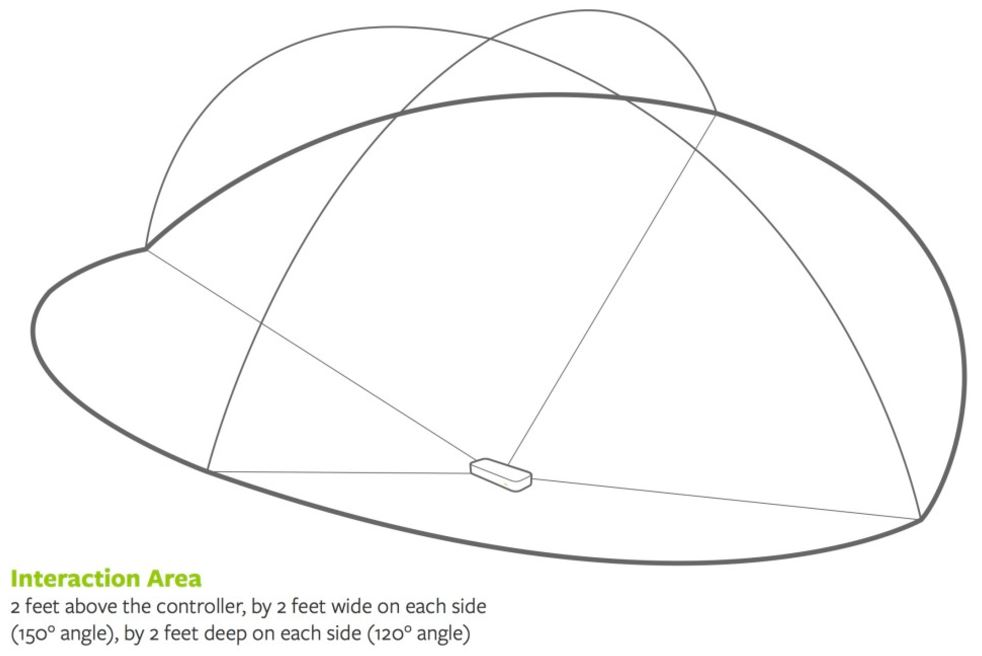
\includegraphics[scale=0.35]{Figures/LeapInteractionArea.JPG}
\caption[Home Screen Layout]{The scene that the user sees intially when they load the application.}
\label{fig:homeScreen}
\end{figure}

The user can click on the Analyze Data button to got 


talk about three scenes and show pics. show what happens where and 
what the typical user would do. 
take data and analyze it for problems. 
and then go fix those problems. 
also save data to csv. read from csv. 
say some things will be dicussed in other sections. 


%------------------------------------------------
%	SECTION 1 User Specific Data Collection
%------------------------------------------------
\section{User Specific Data Collection}


show the 2 figures. explain why you needed ot make users. meeting with clinicians. working product demonstration. agile. as opposed ot waterfall (this should go in conclusion). 

 

%------------------------------------------------
%	SECTION 2 Visual Rotation of Gesture
%------------------------------------------------
\section{Visual Rotation of Gesture}

same as above. 

%------------------------------------------------
%	SECTION 3 Tabular Display of Data
%------------------------------------------------
\section{Tabular Display of Data}

editable picture. show code. 
%------------------------------------------------
%	SECTION 4 Writing and Reading from CSV
%------------------------------------------------
\section{Writing and Reading from CSV}


%------------------------------------------------
%	SECTION 5 Artifacts and Distribution
%------------------------------------------------
\section{Artifacts and Distribution}

%----------------------------------- Leap App Store
\subsection{Leap App Store}

%----------------------------------- IDE Build Process and Batch Script
\subsection{IDE Build Process and Batch Script}


